%!TEX root = ../main.tex

\chapter{Literature Review}\label{cha:literature}

Many extensive literature reviews and surveys have been written on the subject of deep learning.
In 1987, Lippmann reviewed 6 of the most influential Neural Networks of the era \cite{Lippmann_1987}.
In 2001 a review of over 200 applications of neural networks in image processing was published, ranging from preprocessing and feature extraction to segmentation and object recognition \cite{Egmont-Petersen_de_Ridder_Handels_2002}.
More recently, an extensive Survey on Deep Learning in Medical Image Analysis was published \cite{Litjens_Kooi_Bejnordi_Setio_Ciompi_Ghafoorian_van_der_Laak_van_Ginneken_Sanchez_2017}.


\section{Deep Learning}\label{sec:deep_learning_lit}

\subsection{Training Deep Neural Networks}\label{subsec:training}
Due to the size of deep neural networks, and the non-convexity of the parameters, finding good optima has always been a challenge.
Stochastic gradient descent (SGD) has remained a popular strategy for researchers since the 80's although many optimisation algorithms are now used.
These include Adam \cite{Kingma_Ba_2014}, ADADELTA \cite{Zeiler_2012} and AdaGrad \cite{Duchi_Hazan_Singer_2011}.
For all of the optimisers mentioned, one of the main issues during training is choosing an appropriate learning rate.

It has been suggested by Dauphin et al. in \cite{Dauphin_de_Vries_Bengio_2015} that saddle points cause issues during training, not poor local optima.
However, in The Deep Learning Book \cite{Goodfellow-et-al-2016}, Goodfellow et al. prove that although learning is slow around saddle points due to the flatness, gradient based optimisation algorithms are still able to escape.

One possible solution is to use cyclical learning rates instead of a fixed learning rate that decreases over time.
A cycle has a fixed length and the learning rate varies between two sensible boundary values during that cycle.
This helps because if the optimisation gets stuck on a saddle plateau, increasing the learning rate will traverse the plateau quickly.

In Figure \ref{fig:triangular_cyclical_learning_rate} two methods for cyclical learning rates are shown.
Leslie N. Smith propesed these in \cite{Smith_2015}.
On the left plot min and max learning rate are kept the same, wheras on the right the difference is cut in half after each cycle.


\begin{figure}[hbtp!]
    \centering
    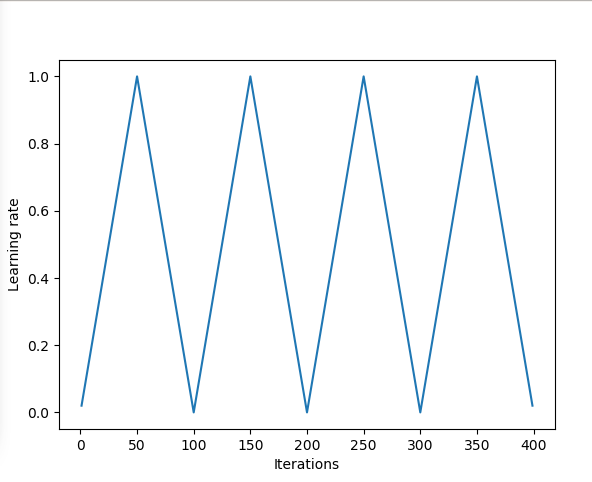
\includegraphics[width=0.45\textwidth]{./img/triangular.png}
    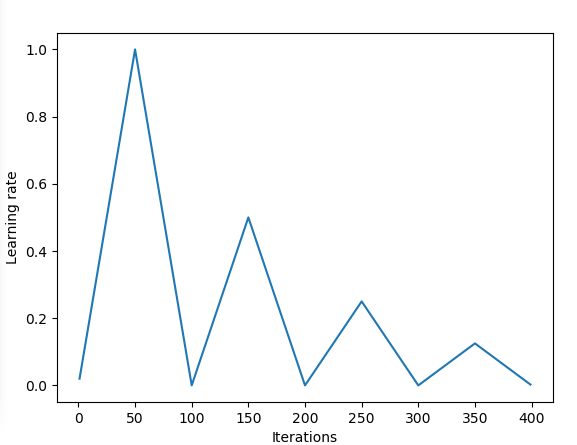
\includegraphics[width=0.45\textwidth]{./img/triangular2.png}
    \caption{Triangular and Triangular2 by Leslie N. Smith \cite{Smith_2015}.}
    \label{fig:triangular_cyclical_learning_rate}
\end{figure}

An alternative was suggested by Loshchilov and Hutter in \cite{Loshchilov_Hutter_2016} called Cosine Annealing.
In this, the learning rate starts at its maximum and decreases to its minimum following the cosine function.
Once the minimum is reached the learning resets to the maximum, there is no increasing phase.
The learning rate $\eta$ is given by:

\begin{equation}
    \eta = \eta_{min} + \frac{1}{2}(\eta_{max} - \eta_{min})(1 + \cos(\frac{T_{cur}}{T_i}\pi)
    \label{eq:cosine_annealing}
\end{equation}

Where $\eta_{min}$ and $\eta_{max}$ are the minimum and maximum learning rates respectively.
$T_{cur}$ is the number of iterations since the previous restart and $T_i$ is the number of iterations within each run.

The authors also suggest making each cycle longer than the last.
This is acheived by increasing $T_i$ after each cycle by a constant factor $T_{mult}$.
Figure \ref{fig:cosine_annealing} shows Cosine Annealing with $T_{mult}=1$ on the left and $T_{mult}=2$ on the right.
In the case of $T_{mult}=1$ this is completely equivalent to Equation \ref{eq:cosine_annealing}.

\begin{figure}[hbtp!]
    \centering
    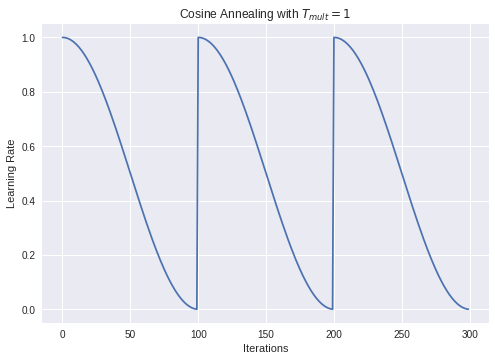
\includegraphics[width=0.45\textwidth]{./img/tmul1.png}
    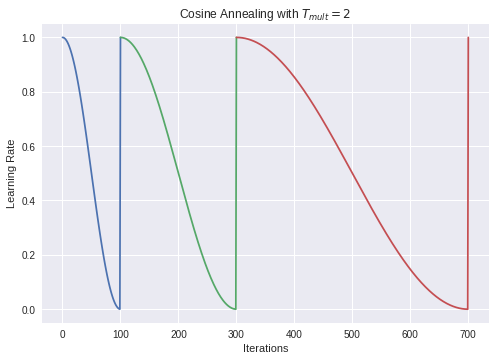
\includegraphics[width=0.45\textwidth]{./img/tmul2.png}
    \caption{Cosine Annealing with $T_{mult}=1$ and $T_{mult}=2$ by Loshchilov and Hutter \cite{Loshchilov_Hutter_2016}.}
    \label{fig:cosine_annealing}
\end{figure}

It is well known that the number of local minima increases exponentially with the number of parameters \cite{Kawaguchi_2016}.
Given that modern neural networks may contain millions of parameters, it is clear that identical architectures with different initialisation will converge to different solutions.
Often local minima have very similar error rates, however the corresponding neural networks will make different mistakes.

This can be exploited using ensembling methods similar to those described by \cite{Caruana_Niculescu-Mizil_Crew_Ksikes_2004}.
In \cite{Huang_Li_Pleiss_Liu_Hopcroft_Weinberger_2017} an ensembling method for Deep Learning is described which they call Snapshot Ensembling.
It extends the work of Loshchilov and Hutter \cite{Loshchilov_Hutter_2016} yet requires no additional training time.
This was achieved by saving the model weights at the end of each learning rate cycle ie. taking a snapshot.
Each time the learning rate is reset the neural net converges to a new local optima producing a substantially different model.
In the right hand side of Figure \ref{fig:cosine_annealing}, each coloured sections corresponds to the model converging to a different local minima.
The saved models can then be used as an ensemble at prediction time.


\subsection{Recent Developments}\label{subsec:recent_improvements}

In this section, an overview of some more recent developments will be given.
First, an extension of learning rate cycling and ensemble methods will be discussed.
Finally, Hinton's breakthrough regarding Capsule Networks will also be presented.

In \cite{Keskar_Mudigere_Nocedal_Smelyanskiy_Tang_2016} it is suggested that convergence to sharp minima leads to poor generalisation for deep learning.
The motivation for this suggestion is that the training loss surface and test loss surface will be similar but not exactly the same; one may be shifted when compared to the other.
For sharp minima, a point with low loss during training may produce large loss during testing due to this shift.
Whereas for a wide minima, the effect of this shift would be reduced.
This is shown in Figure \ref{fig:wide_optima} where a sharp and wide minima are compared.

\begin{figure}[hbtp!]
    \centering
    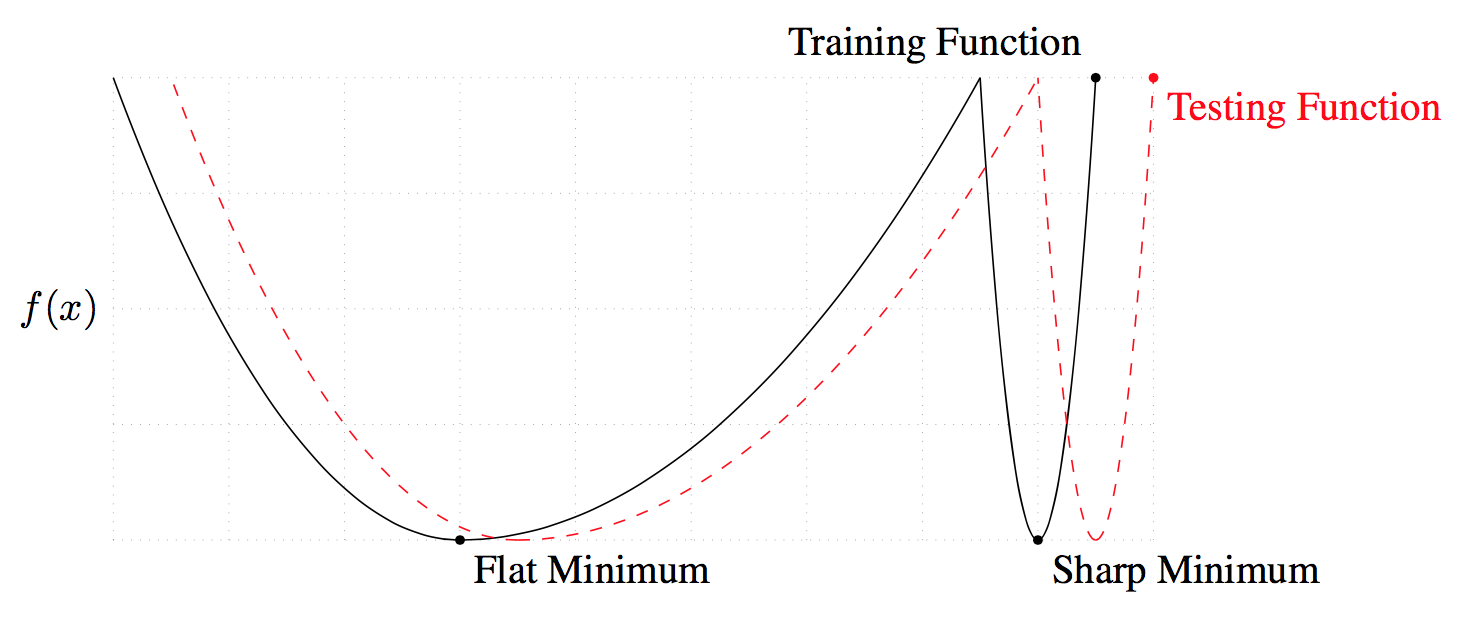
\includegraphics[width=\textwidth]{./img/Wide_optima.png}
    \caption{A Conceptual Sketch of Flat and Sharp Minima. The Y-axis indicates value of the loss function and the X-axis the variables (parameters) \cite{Keskar_Mudigere_Nocedal_Smelyanskiy_Tang_2016}}
    \label{fig:wide_optima}
\end{figure}

Numerical evidence is then given that supports this view and several attempts to address the problem are presented.
However, initial results suggest that whilst these strategies do lead to better generalisation, they still converge to sharp minima.
The next two methods are able to produce wide optima, and thus generalise very well at test time.

Fast Geometric Ensembling (FGE) is very similar to Snapshot Ensembling as described in Section \ref{sec:deep_learning_lit}.
The main differences are that it uses a piecewise linear cyclical learning rate (instead of cosine) and a much shorter cycle length.
A short cycle make seem intuitively wrong, because the saved models will not differ from each other much and therefore provide no benefit when taken as an ensemble.
However, in \cite{Garipov_Izmailov_Podoprikhin_Vetrov_Wilson_2018} it is shown that there exist connected paths of low loss between sufficiently different models and that it is possible to travel along those paths in small steps.
Thus the models encountered along the path will be different enough to allow ensembling them with good results.

Figure \ref{fig:FGE_shortest_path} demonstrates this concept on the cross-entropy loss surface of ResNet-164 on CIFAR-100.
The vertical axis changes between panels as we change planes.
The left plane shows three optima for independently trained networks.
These three optima are all isolated which agrees with standard intuition.
However, the middle and right panels show two different paths of near-constant loss, discovered by FGE training procedure.
The endpoints of the path correspond to two independently trained networks that coincide with the two lower optima in the left panel.
Notice that in each panel a direct linear path between each optima would incur high loss.

\begin{figure}[hbtp!]
    \centering
    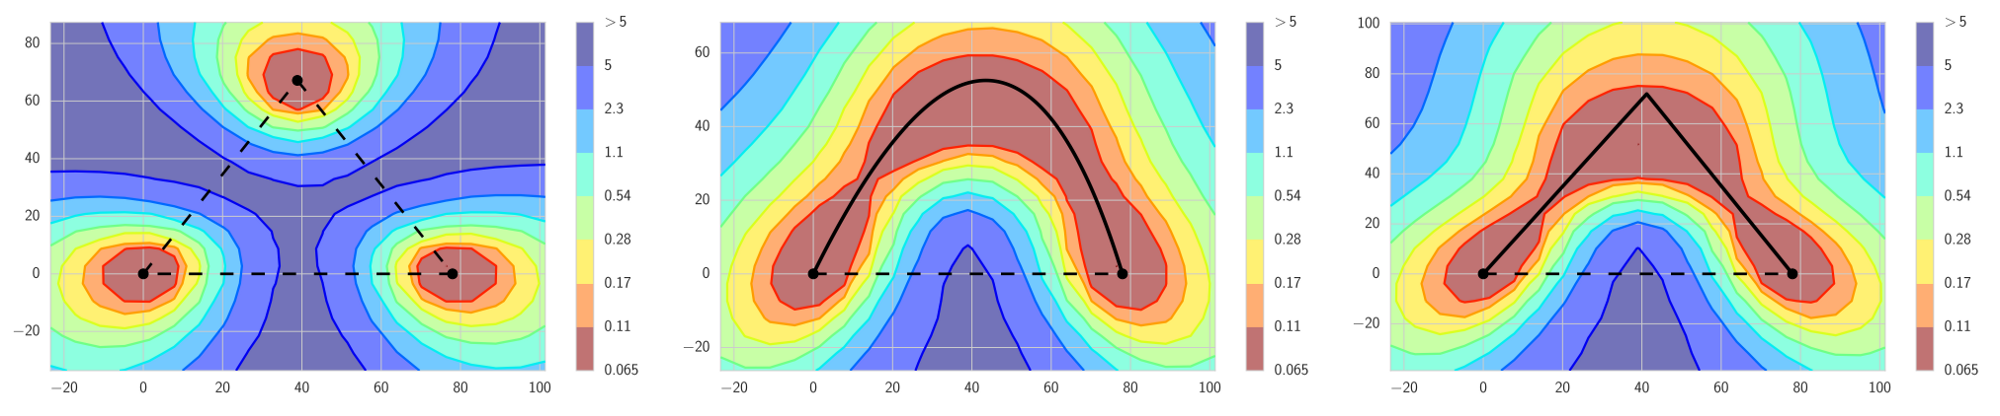
\includegraphics[width=\textwidth]{./img/FGE.png}
    \caption{The cross-entropy loss surface of a deep residual network (ResNet-164) on CIFAR-100, as a function of network weights in a two-dimensional subspace \cite{Garipov_Izmailov_Podoprikhin_Vetrov_Wilson_2018}.}
    \label{fig:FGE_shortest_path}
\end{figure}

FGE shows improvement on Snapshot Ensembling and due to the shorter learning rate cycle it is also faster to train.
However, to obtain the superior performance of FGE or Snapshort Ensembling many different models must be stored.
Also, predictions must be made by each model which are then averaged together, implying increased computations at test time.
In \cite{Izmailov_Podoprikhin_Garipov_Vetrov_Wilson_2018}, a training method is outlined that avoids this issue whilst maintaining comparable performance.

The methodologies discussed so far have been ensembles in model space; they use the predictions of several models to produce a final result.
In \cite{Izmailov_Podoprikhin_Garipov_Vetrov_Wilson_2018}, weights are averaged instead of model predictions.
It is shown that the Stochastic Weight Averaging (SWA) procedure finds much wider optima than SGD and approximates FGE.

The method only requires two models to be stored.
The first, $w_{SWA}$ maintains a running average of model weights.
The second, $w$ traverses the weight space.
The running average is then updated periodically by the rule:

\begin{equation}
    w_{SWA} \leftarrow \frac{w_{SWA} \cdot n_{models} + w}{n_{models} + 1}
    \label{eq:swa}
\end{equation}

Where $n_{models}$ is the number of models captured so far.
If using a cyclical learning rate, $w_{SWA}$ should be updated each time the learning rate reaches the minimum value.
Otherwise it should be updated at the end of each epoch of training (or some multiple of epochs).

In Figure \ref{fig:SWA} SWA and SGD are compared.
The left panel shows three sampled FGE solutions and the corresponding SWA solution that has been averaged in weight space.
The right panel shows the train loss surface and corresponding convergence of both SWA and SGD.
They were started from the same initialisation of SGD after 125 epochs.
The middle panel shows the exact same models but for the test error.
It can be seen that whilst SGD performs better on the training set, SWA is able to generalise more.

\begin{figure}[hbtp!]
    \centering
    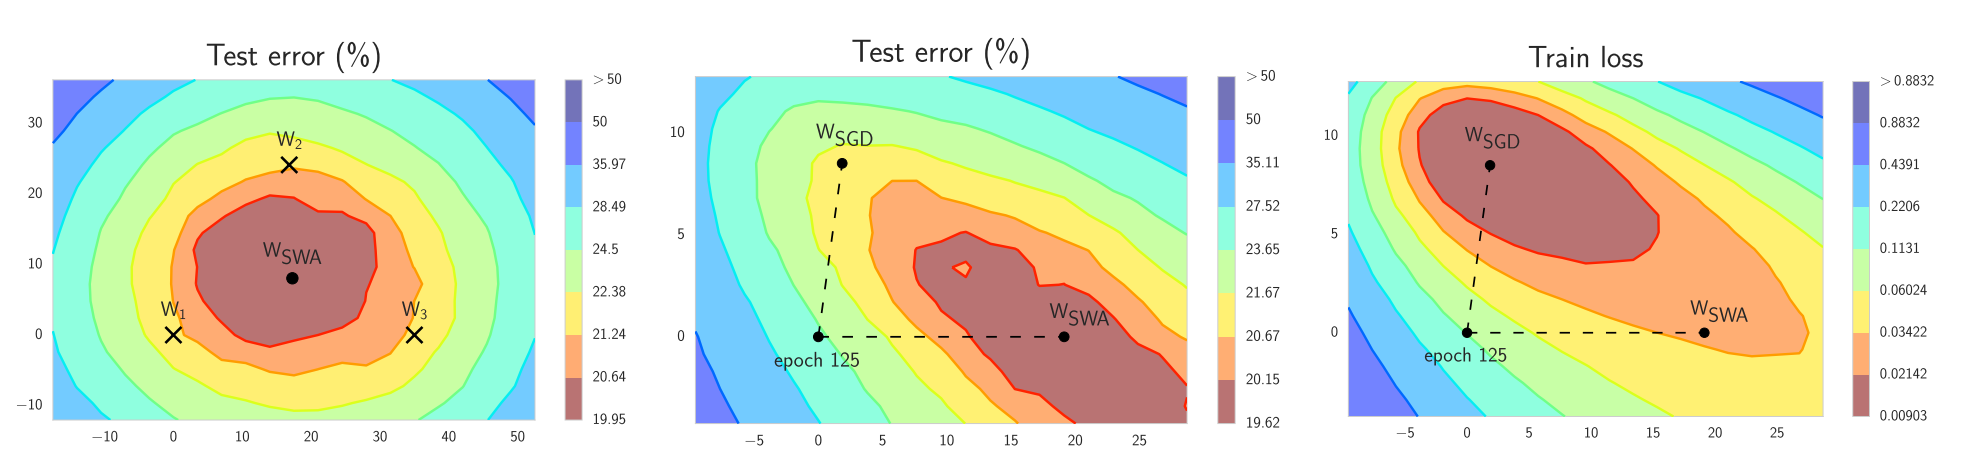
\includegraphics[width=\textwidth]{./img/SWA.png}
    \caption{Illustrations of SWA and SGD with a Preactivation ResNet-110 on CIFAR-100. \cite{Izmailov_Podoprikhin_Garipov_Vetrov_Wilson_2018}}
    \label{fig:SWA}
\end{figure}


% % TODO Capsule
% In late 2017, Hinton outlined a method for training capsule based methods.
% This is something he'd been thinking about for years.
% It learns pose representations of objects. \cite{Hinton_Sabour_Frosst_2018, Sabour_Frosst_Hinton_2017}





\section{Deep Learning in Medicine}\label{deep_learning_medic_lit}
% TODO section on deep learning in medicine

In \cite{Ching_Himmelstein_Beaulieu-Jones_Kalinin_Do_Way_Ferrero_Agapow_Zietz_Hoffman_et_al_2018} a comprehensive overview of the opportunities and obstacles for deep learning in biology and medicine is given.
Ching et al. discuss the many different areas where deep learning could be utilised.
This includes:

\begin{itemize}
    \item Disease/patient categorisation eg. classifying breast cancer
    \item Biological study eg. gene and protein behaviour prediction
    \item Treatment of patients eg. predicting drug targets and responses
\end{itemize}

They also cover some of the challenges facing deep learning:

\begin{itemize}
    \item Generating ground truth can expensive
    \item Data sharing is hampered by standardisation and privacy considerations
    \item Discrimination and `right to an explanation' laws
\end{itemize}

\subsection{Deep Learning in Medical Image Analysis}\label{deep_learning_medical_image}

Deep learning algorithms and particularly convolutional networks have become an increasingly popular choice for medical image analysis.
In \cite{Litjens_Kooi_Bejnordi_Setio_Ciompi_Ghafoorian_van_der_Laak_van_Ginneken_Sanchez_2017}, over 300 contributions to this field are summarised.
The use of deep learning for image classification, object detection and segmentation are all reviewed.
Also overviews of anatomical areas are provided, including neuro, retinal, pulmonary, digital pathology, breast, cardiac, abdominal and musculoskeletal.

One of the main challenges for deep learning when applied to medical images is the absence of large sets of labelled training data.
In \cite{Ronneberger_Fischer_Brox_2015}, Ronneberger introduces the U-Net architecture (see Figure \ref{fig:unet}) which is comprised of a contracting path, a symmetric expanding path and skip connections between them.

\begin{figure}[hbtp!]
    \centering
    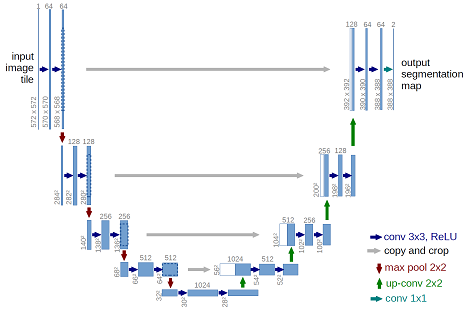
\includegraphics[width=\textwidth]{./img/u-net-architecture.png}
    \caption{U-net architecture. Blue boxes denote multi-channel feature maps and the number of channels is denoted on top of the box. \cite{Ronneberger_Fischer_Brox_2015}}
    \label{fig:unet}
\end{figure}

This method won several competitions including the ISBI challenge for segmentation of neuronal structures and the ISBI cell tracking challenge.
These competitions provided only 30 and 35 training images respectively.
The idea of U-Nets was taken further in \cite{Cicek_Abdulkadir_Lienkamp_Brox_Ronneberger_2016} where it was generalised to 3D images and used for segmentation of kidneys.
In \cite{Iglovikov_Shvets_2018}, Iglovikov and Shvets show how the use of a pre-trained encoder in a U-Net architecture can improve performance.
However, this was not applied to a medical image scenario.

There have been many cases of neural networks equaling the success of expert doctors in image analysis.
Some notable examples are \cite{Liu_Gadepalli_Norouzi_Dahl_Kohlberger_Boyko_Venugopalan_Timofeev_Nelson_Corrado_et_al_2017, Esteva_Kuprel_Novoa_Ko_Swetter_Blau_Thrun_2017}.
In \cite{Liu_Gadepalli_Norouzi_Dahl_Kohlberger_Boyko_Venugopalan_Timofeev_Nelson_Corrado_et_al_2017} a framework to aid breast cancer metastasis detection is given.
They used an Inception architecture \cite{Russakovsky_Deng_Su_Krause_Satheesh_Ma_Huang_Karpathy_Khosla_Bernstein_et_al_2015} which performed so well that it found two slides in the Camelyon16 \cite{Camelyon16} training set that were labelled incorrectly.
An Inception architecture was also used in  \cite{Esteva_Kuprel_Novoa_Ko_Swetter_Blau_Thrun_2017} to produce dermatologist level classification skin cancer.
In this case the CNN had been pretrained on 1.28 million images.

% \subsection{Adversarial Networks}

% The subject of adversarial Networks is very popular within the deep learning community.
% Adversarial Nets \cite{Finlayson_Chung_Kohane_Beam_2018}
